% !TeX root = main.tex

\section{Approach}

\begin{frame}{\insertsection}
	\begin{itemize}
		\setlength{\itemsep}{8pt}
		\item \textit{Continuous detection} \onslide<2->\\
			$\rightarrow$ \textbf{Index-based approach}\onslide<3->
		\item \textit{High accuracy}\onslide<4->\\
			$\rightarrow$ \textbf{Indexing History}\onslide<5->
		\item \textit{Huge amount of open source code}\onslide<6->\\
			$\rightarrow$ \textbf{Server-client architecture}\onslide<7->
		\item \textit{Confidentiality}\onslide<8->\\
			$\rightarrow$ \textbf{Sending hashes instead of source code}\onslide<9->
		\item \textit{High number of lookup-requests}\onslide<10->\\
			$\rightarrow$ \textbf{Filtering hashes on client}
	\end{itemize}
\end{frame}

\subsection{Architecture}
\begin{frame}{\insertsubsection}
	\only<1>{\includegraphics[width=\linewidth]{fig/architecture_overview_client_server.pdf}}
	\only<2>{\includegraphics[width=\linewidth]{fig/architecture_overview_server.pdf}}
\end{frame}

\subsection{Index Creation}
\subsubsection{Normalization}
\begin{frame}{\insertsubsection}{\insertsubsubsection}
	\begin{center}
		\includegraphics[width=0.9\linewidth]{fig/normalization_1.pdf}
	\end{center}
	\begin{itemize}
		\small
		\item Removes formatting, comments, access modifiers, brackets, import statements, ...
		\item Focus on features and properties relevant for comparing copied code
	\end{itemize}

	\note{
		\begin{itemize}
			\item Entfernt Formattierung, comments, access modifiers, brackets, import statements, keywords like final/static
			\item Übriges: "Fingerabdruck" (Struktur, Variablennamen, Literale, ...)
		\end{itemize}
	}
\end{frame}

\subsubsection{Hashing chunks}
\begin{frame}{\insertsubsection}{\insertsubsubsection}
	\begin{center}
		\includegraphics[width=0.9\linewidth]{fig/normalization_2.pdf}
	\end{center}
	\begin{itemize}
		\item Splitting normalized code into statements
		\item Group into chunks of 5 statements
		\item Location of chunk is stored in index
		\item Hash is used as key
	\end{itemize}
	\note{
		\begin{itemize}
			\item Index is key value store
		\end{itemize}
	}
\end{frame}

\subsubsection{History Analysis}
\begin{frame}{\insertsubsection}{\insertsubsubsection}
	\begin{center}
		\includegraphics[width=\linewidth]{fig/history_analysis.pdf}
	\end{center}
	
	\begin{itemize}
		\item Analyzing history relevant to find old versions of a file
		\item Using git tags as reference points
		\item Re-indexing changed files between two versions
	\end{itemize}
\end{frame}

\begin{frame}{\insertsubsection}
\only<3>{\includegraphics[width=\linewidth]{../written/figures/architecture_overview.pdf}
\begin{description}
	\small
	\item[Target System] System on client which should be scanned for copied code
	\item[Reference System] Open source software system on server
\end{description}
}
\note{
\begin{itemize}
	\item TODO
\end{itemize}
}
\end{frame}

\subsection{Searching for Copied Code}
\begin{frame}{\insertsubsection}
	\includegraphics[width=\linewidth]{../written/figures/searching_copied_code.pdf}
\end{frame}

\subsubsection{Hash Filter}
\begin{frame}{\insertsubsection}{\insertsubsubsection}
\textbf{Problem:} Lots of request have to be sent to server\\
\pause
\vspace{2mm}
\textbf{Solution:} Bloom filter on client side
\vspace{2mm}
\begin{itemize}
	\small
	\item Data structure, calculated on server, downloaded to client
	\item Client can decide whether a hash is part of the index with very small false positive probability (0,01\%)
	\item Fraction in size compared to the index database\\ (37 GB $\rightarrow$ 200 MB)
	\item Reduces number of requests to a fraction
\end{itemize}
\end{frame}

%TODO aggregation?
